
%(BEGIN_QUESTION)
% Copyright 2010, Tony R. Kuphaldt, released under the Creative Commons Attribution License (v 1.0)
% This means you may do almost anything with this work of mine, so long as you give me proper credit

Dette pH-overvåkingssystemet utløser alarm dersom pH-verdien til prosessvannet i nøytraliseringstanken driver forbi en av to terskelverdier (trip-verdier):

$$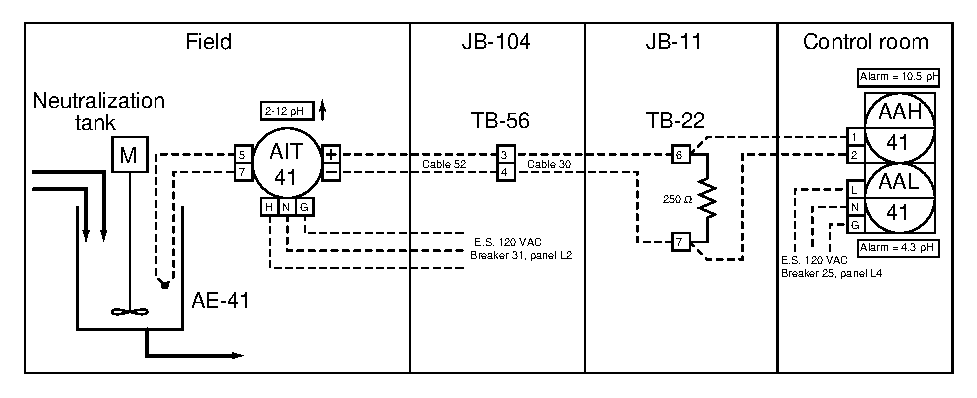
\includegraphics[width=15.5cm]{i00239x01.eps}$$

Svar på følgende spørsmål om dette pH-alarmsystemet:

\vskip 10pt

\begin{itemize}
\item{} Hvis en leder løsner ved TB56-4 og skaper en ``åpen'' feil i sløyfekretsen, beskriv hva som skjer i alarmenheten (AAH, AAL-41), samt hvor du forventer å måle spenning i sløyfekretsen og hvor du forventer å måle {\it ingen} spenning.
\vskip 20pt
\item{} Hvis sikring/vern \#25 i panel L4 plutselig løser ut, hva vil skje i dette systemet?  Vil en operatør fortsatt kunne lese pH-verdien i nøytraliseringstanken?
\vskip 20pt
\item{} Hvis det oppstår brann nær røret hvor kabel 52 ligger, slik at plastisolasjonen rundt lederne i kabel 52 smelter og dermed kortslutter lederne, hva vil skje i systemet?  Hvor forventer du å måle spenning i sløyfekretsen, og hvor forventer du å måle {\it ingen} spenning?  Hvor forventer du å måle strøm i sløyfekretsen, og hvor forventer du å måle {\it ingen} strøm?
\vskip 20pt
\item{} Beregn sløyfestrømmen når pH måles til 6.8 i nøytraliseringstanken.
\end{itemize}



\vskip 20pt \vbox{\hrule \hbox{\strut \vrule{} {\bf Forslag til sokratisk diskusjon} \vrule} \hrule}

\begin{itemize}
\item{} For dem som har studert pH-måling: forklar hvorfor pH-``nøytralisering'' er en viktig reguleringsprosess i industrien.
\item{} Hvordan kan vi se i dette diagrammet om 4-20 mA-utgangen til transmitter AIT-41 er {\it aktiv} eller {\it passiv} (dvs. {\it sourcing} eller {\it sinking})?
\end{itemize}

\underbar{file i00239}
%(END_QUESTION)





%(BEGIN_ANSWER)

\noindent
{\bf Delvis svar:}

\begin{itemize}
\item{} Hvis en leder løsner ved TB56-4 og skaper en ``åpen'' feil i sløyfekretsen, beskriv hva som skjer i alarmenheten (AAH, AAL-41), samt hvor du forventer å måle spenning i sløyfekretsen og hvor du forventer å måle {\it ingen} spenning.  {\it AAL vil trippe (men ikke AAH), og vi forventer å måle spenning mellom lederne i kabel 52, men ikke mellom lederne i kabel 30.}
\vskip 10pt
\item{} Hvis det oppstår brann nær røret hvor kabel 52 ligger, slik at lederne i kabel 52 {\it kortsluttes}, hva vil skje i dette systemet?  Hvor forventer du å måle spenning i sløyfekretsen, og hvor forventer du å måle {\it ingen} spenning?  Hvor forventer du å måle strøm i sløyfekretsen, og hvor forventer du å måle {\it ingen} strøm?  {\it AAL vil trippe (men ikke AAH), og vi forventer å måle ingen spenning noe sted i sløyfekretsen.  Vi vil imidlertid fortsatt ha strøm ved terminalene på AIT-41-transmitteren (men ingen strøm til høyre for kortslutningen).}
\end{itemize}

%(END_ANSWER)





%(BEGIN_NOTES)

\begin{itemize}
\item{} Hvis en leder løsner ved TB56-4 og skaper en ``åpen'' feil i sløyfekretsen, beskriv hva som skjer i alarmenheten (AAH, AAL-41), samt hvor du forventer å måle spenning i sløyfekretsen og hvor du forventer å måle {\it ingen} spenning.  {\it AAL vil trippe (men ikke AAH), og vi forventer å måle spenning mellom lederne i kabel 52, men ikke mellom lederne i kabel 30.}
\vskip 10pt
\item{} Hvis sikring/vern \#25 i panel L4 plutselig løser ut, hva vil skje i dette systemet?  Vil en operatør fortsatt kunne lese pH-verdien i nøytraliseringstanken?  {\it Begge alarmer blir døde, men indikerende transmitter (AIT-41) vil fortsatt indikere pH korrekt.}
\vskip 10pt
\item{} Hvis det oppstår brann nær røret hvor kabel 52 ligger, slik at lederne i kabel 52 {\it kortsluttes}, hva vil skje i dette systemet?  Hvor forventer du å måle spenning i sløyfekretsen, og hvor forventer du å måle {\it ingen} spenning?  Hvor forventer du å måle strøm i sløyfekretsen, og hvor forventer du å måle {\it ingen} strøm?  {\it AAL vil trippe (men ikke AAH), og vi forventer å måle ingen spenning noe sted i sløyfekretsen.  Vi vil imidlertid fortsatt ha strøm ved terminalene på AIT-41-transmitteren (men ingen strøm til høyre for kortslutningen).}
\vskip 10pt
\item{} Hvis pH = 6.8, strøm = 11.68 mA
\end{itemize}
















\vskip 20pt \vbox{\hrule \hbox{\strut \vrule{} {\bf Virtuell feilsøking} \vrule} \hrule}

Denne oppgaven egner seg godt til en ``virtuell feilsøking''-øvelse.  Presenter diagrammet for studentene, og bestem deg først for en konkret feil i systemet.  Presenter deretter ett eller flere symptomer på feilen (noe en operatør eller annen bruker ville kunne observere).  Studentene foreslår så diagnostiske tester for å identifisere type og plassering av feilen, som om de var teknikere som feilsøkte problemet.  Din jobb er å gi resultatene av hver foreslåtte test, og dokumentere dem slik at alle studentene ser dem.

Under og etter øvelsen er det nyttig å stille oppfølgingsspørsmål som:

\begin{itemize}
\item{} Hva forteller resultatet av siste diagnostiske test om feilen?
\item{} Anta at resultatet av siste diagnostiske test var annerledes.  Hva ville det i så fall fortalt om feilen?
\item{} Er siste diagnostiske test den beste testen vi kan gjøre?
\item{} Hva ville vært ideell testrekkefølge for å diagnostisere problemet på færrest mulig trinn?
\end{itemize}


\vfil \eject

\noindent
{\bf Forberedelsesquiz:}

Anta at en tekniker bryter 4-20 mA-sløyfen ved TB-56 for å måle strøm.  Hvilken effekt vil inntreffe umiddelbart?

$$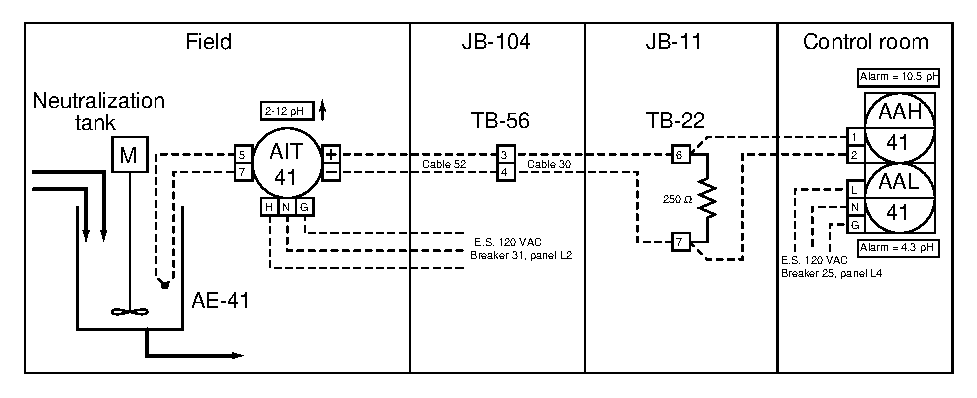
\includegraphics[width=15.5cm]{i00239x01.eps}$$

\begin{itemize}
\item{} Lav pH-alarm aktiveres umiddelbart
\vskip 5pt 
\item{} Høy pH-alarm aktiveres umiddelbart
\vskip 5pt 
\item{} pH-transmitteren mister umiddelbart strøm
\vskip 5pt 
\item{} Miksormotoren stopper umiddelbart
\vskip 5pt 
\item{} pH-verdien i vannet begynner å stige
\vskip 5pt 
\item{} pH-verdien i vannet begynner å synke
\end{itemize}


\vfil \eject

\noindent
{\bf Forberedelsesquiz:}

Beregn pH-verdien i vannet i denne nøytraliseringstanken dersom analysatorens strømsignal er 17.5 milliampere.

$$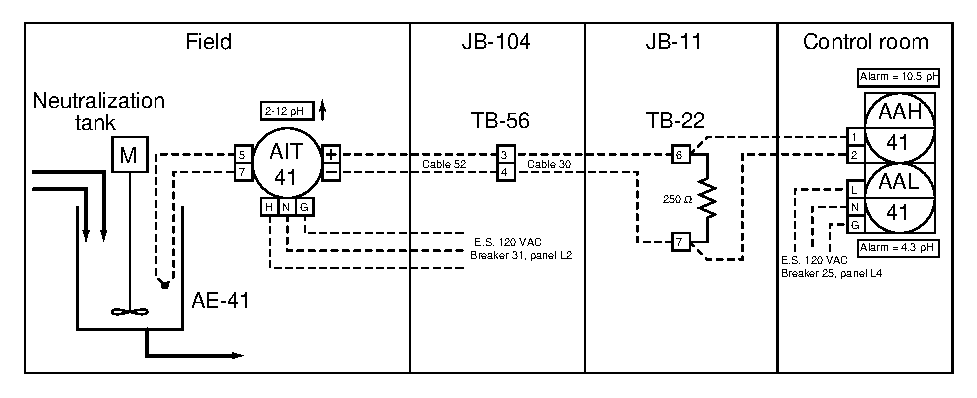
\includegraphics[width=15.5cm]{i00239x01.eps}$$

\begin{itemize}
\item{} 12.08 pH
\vskip 5pt 
\item{} 8.44 pH
\vskip 5pt 
\item{} 10.94 pH
\vskip 5pt 
\item{} 11.69 pH
\vskip 5pt 
\item{} 10.44 pH
\vskip 5pt 
\item{} 11.44 pH
\end{itemize}


%INDEX% Basics, 4-wire self-powered transmitter: circuit analysis
%INDEX% Measurement, analytical: pH
%INDEX% Process: water pH neutralization (generic)

%(END_NOTES)
